\chapter{LHC-ATLAS実験}
\label{chapter2}

LHC-ATLAS 実験とは、LHC (Large Hadron Collider)を用いた高エネルギーの陽子–陽子衝突によって生成された粒子を ATLAS (A Troidal LHC ApparatuS) 検出器によって検出し、標準模型の精密測定や新粒子探索などを行う実験である。
LHCでは高エネルギー状態の陽子を衝突させることにより、TeV スケールまでの物理事象を広く調べることを可能にしている。
LHC は 2018 年に Run-2 を終了し、2019 年から 2021 年にかけて LHC 及び ATLAS 検出器のアップグレードが行われ、2022 年から Run-3 が開始された。

本章では、Run-3におけるLHC及びATLAS検出器の概要とATLAS実験で採用されているトリガーシステムについて述べる。

\section{LHC加速器}
\label{section2-1}
Large Hadron Collider (LHC)は、スイスのジュネーブ郊外にある欧州素粒子原子核研究機構 (CERN)の地下に建設された周長約 27 km の世界最大の大型ハドロン衝突型加速器である。LHCの全体像を図\ref{fig:LHC加速器}に示す。
LHC は14 TeV の重心系エネルギー、$1\times10^{34}$ cm$^{-2}$s${^-1}$の瞬間ルミノシティで陽子-陽子衝突が可能なように設計されている。LHCの衝突実験で使用される陽子ビームはバンチと呼ばれる 10${^11}$ 個の陽子のかたまりで構成されており、LHCの一周あたりに 25 ns のバンチ間隔で入射されているため、陽子-陽子衝突を起こす際の各バンチの衝突頻度は 40 MHz となっている。
Run-3では陽子-陽子衝突の重心系エネルギーを 13.6 TeVに増強し、瞬間ルミノシティ 2.0$\times$10$^{34}$ cm$^{−2}$s$^{−1}$ での運転を行い、Run-2 で取得したデータと合わせて積分ルミノシティで 350 fb$^{−1}$ のデータを取得する予定である。

\begin{figure}[tb]
  \centering
  \includegraphics[clip]{fig/2/accel_complex-v2022_complex.png}
  \caption{LHC加速器の概略図}
  \label{fig:LHC加速器}
\end{figure}


LHCでは陽子を衝突させる前に、いくつかの前段加速器を使用しTeVスケールの高エネルギーまで加速している。
初めに水素原子に強い電場をかけることで、衝突実験で使用する陽子を得る。
この陽子は線形加速器である LINAC2 で 50MeV まで加速される。次に、Proton Synchrotron Booster (PSB) で1.4GeVまで加速された後、Proton Synchrotron (PS) で陽子を26GeVまで加速し、40MHzのバンチ構造を持った陽子ビームを形成する。
その後、Super Proton Synchrotron (SPS) で450GeVまで加速された後、陽子ビームはLHCに入射され最大で7 TeV まで加速される。
LHCは陽子ビームが反対方向に周回するための2つのリングから構成されており、4か所ある衝突点にそれぞれ検出器が設置されている。
その衝突点の一つに ATLAS 検出器が設置され、陽子同士の衝突から生成される粒子を検出する。
他3箇所にも検出器が設置されており、それぞれCMS(Compact Muon Solenoid)、LHCb (Large Hadron Collider b)、ALICE (A Large Ion Collider Experiment)である。
ATLAS と CMS の2つの検出器は、標準模型の検証から標準模型を超える現象の探索まで可能な汎用検出器である。
LHCb と呼ばれる検出器は、B-ハドロン系の物理を研究するために設計されたものである。
最後の ALICE は、QCD 現象を探るために重イオン衝突の研究に最適化された検出器である。

\section{LHC-ATLAS 実験}
\label{section2-2}
本節では、LHC-ATLAS 実験で使用される ATLAS 検出器とトリガーシステムについて説明する。

\subsection{ATLAS検出器}
ATLAS検出器は、LHCの衝突点の1つに設置された、直径25m、長さ44mの円筒形の大型汎用検出器である。全体像を図\ref{fig:ATLAS検出器}に示す。
ATLAS検出器は複数の検出器を組み合わせて構成されており、内側から大きく分けて内部飛跡検出器、カロリメータ、ミューオン検出器といった検出器が設置されている。また、内部飛跡検出器とカロリメータの間には超電導ソレノイド磁石、カロリメータの外側にはトロイド磁石がそれぞれ設置されている。
これらの検出器から得られる情報を組み合わせることで、粒子識別や粒子のエネルギーなどの測定を行っている。
以下では各検出器の概要について述べる。

\begin{figure}[tb]
  \centering
  \includegraphics[clip,width=14cm]{fig/2/0803012_01.jpg}
  \caption{ATLAS検出器の全体図}
  \label{fig:ATLAS検出器}
\end{figure}


\subsection{ATLAS検出器における座標系}
ATLAS実験では図\ref{fig:a}に示すような直行座標系と円筒座標系が使用されている。直行座標系では、検出器の中心を原点として、ビーム軸に沿ってz軸を取る。ビーム軸に垂直な平面をx-y平面としたときに、加速器の中心方向を正とするx軸及び、地面に対して垂直方向上向きを正とするy軸を設定する。円筒座標系では、ビーム軸に沿ったz軸に対し、動径方向を$R$、ビーム軸周りの角度を方位角$\phi$、ビーム軸からの角度を極角$\theta$としている。
ATLAS 検出器では z 軸が正の側を A-side、負の側を C-side と定義している。

また、ATLAS実験で使用される座標系として、
\begin{equation}
 \eta=-ln(tan\frac{\theta}{2})
 \label{ラピディティ}
\end{equation}

と定義される擬ラピディティ$\eta$が用いられる。

ATLAS 検出器は円筒形をしており、側面部分と底面部分に配置される検出器を分けて考えるため、$|\eta| < 1.0$ の側面部分をバレル領域、$|\eta| > 1.0$ の底面部分をエンドキャップ領域と呼ぶ。



\begin{figure}[tb]
  \centering
  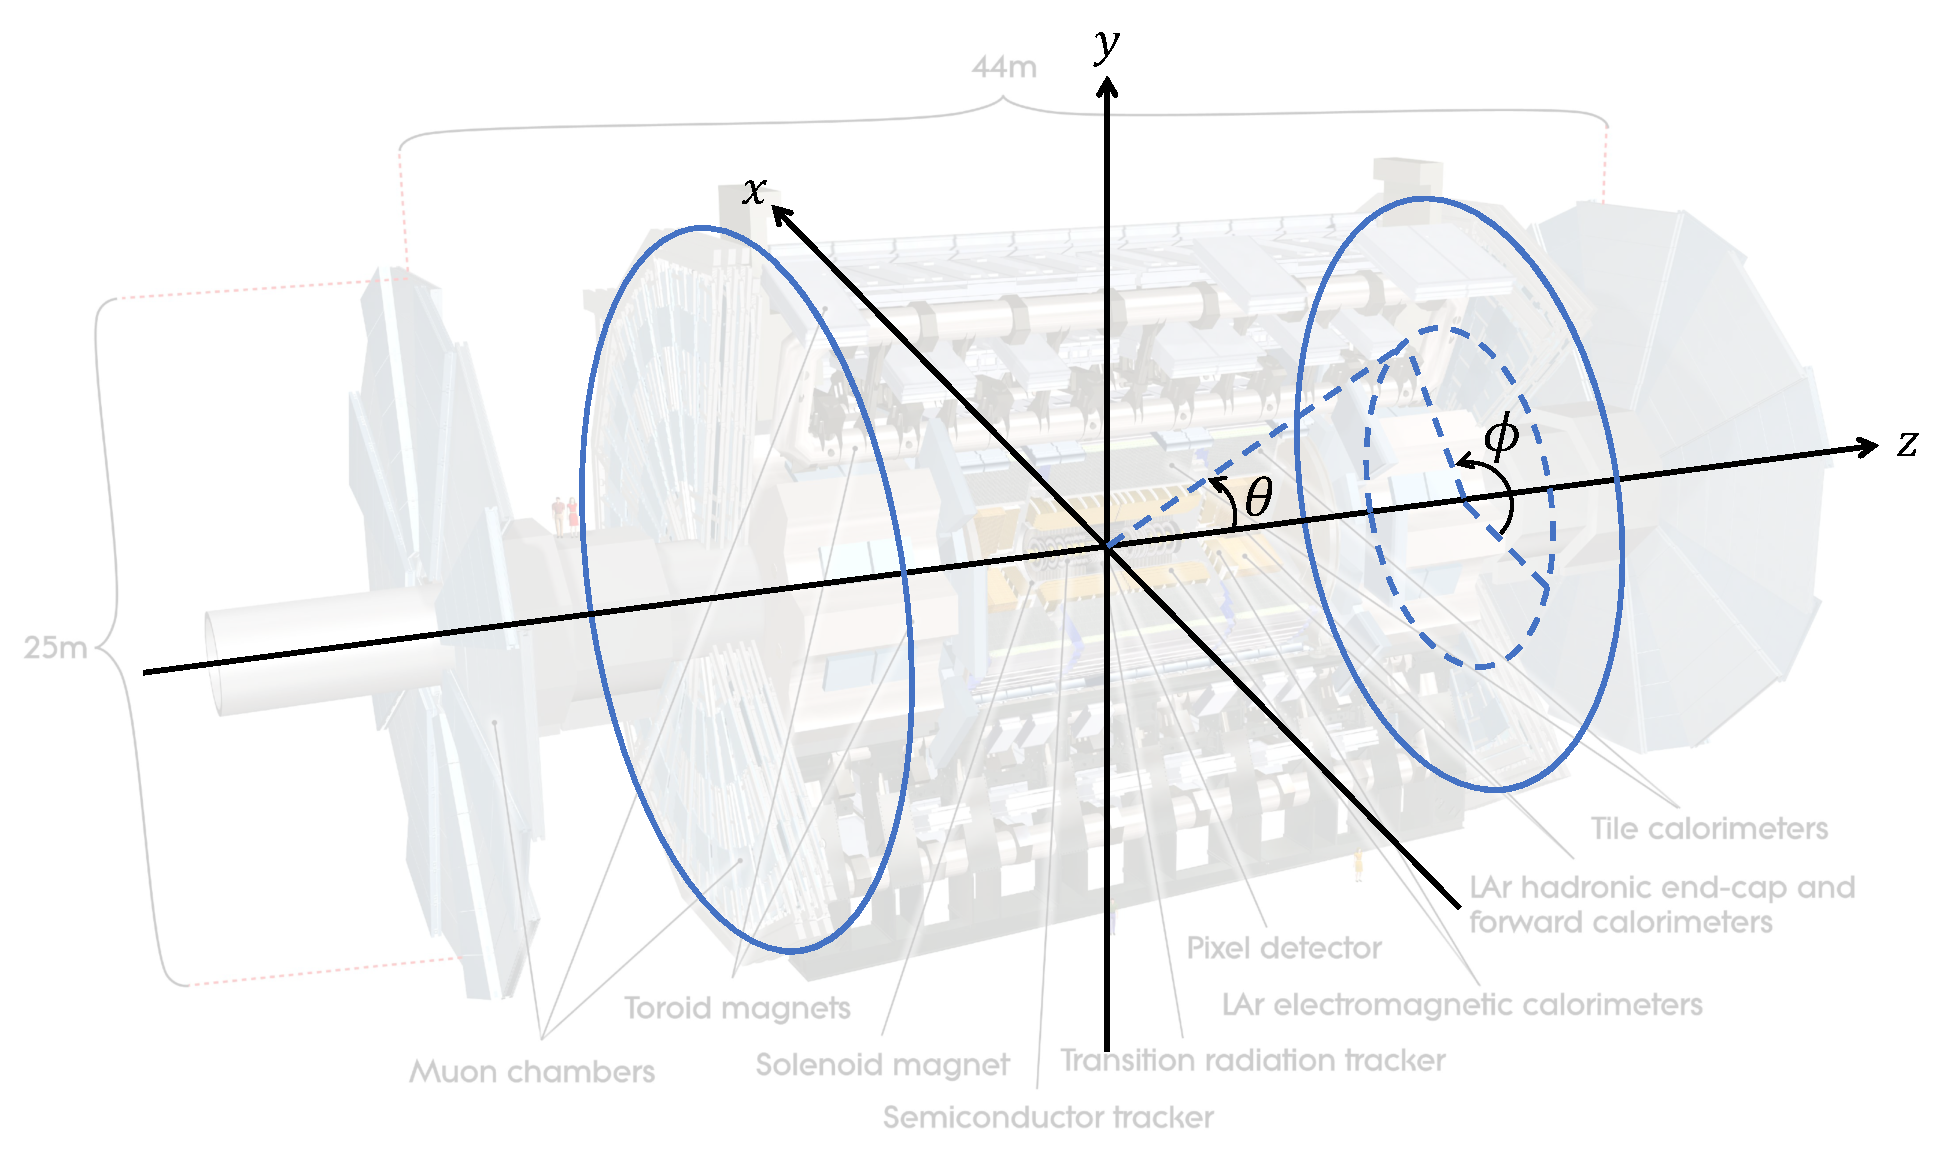
\includegraphics[clip, width=14cm]{fig/2/atlas_coordinate_fix.pdf}
  \caption{ATLAS検出器における座標系}
  \label{fig:a}
\end{figure}

\subsection{マグネットシステム}
ATLAS 実験では、荷電粒子の運動量測定のために超伝導磁石を用いている。超伝導磁石は 2 種類あり、1 つは衝突点付近で発生した荷電粒子の運動量測定のために用いられるソレノイド磁石であり、もう 1 つはミューオンの運動量測定のために用いられるトロイド磁石である。トロイド磁石はバレル部とエンドキャップ部に分けられ、それぞれ$\phi$ 方向に等間隔で 8 つずつ配置されている。ただし、バレル部とエンドキャップ部での磁場の干渉を考慮して、エンドキャップ部のトロイド磁石はバレル部に対して 22.5 度回転した状態で配置されている。

\subsection{内部飛跡検出器}
内部飛跡検出器は衝突点で発生した荷電粒子の飛跡を測定する。その際、荷電粒子の飛跡はソレノイド磁石によって曲げられる。この飛跡は荷電粒子の運動量の算出に用いられる。
内部飛跡検出器は内側から Insertable B-Layer (IBL)、ピクセル検出器、Semiconductor Tracker (SCT)、Transition Radiation Tracker (TRT) で構成されている。


\begin{figure}
    \centering
    \begin{minipage}[b]{0.4\linewidth}
        \centering
        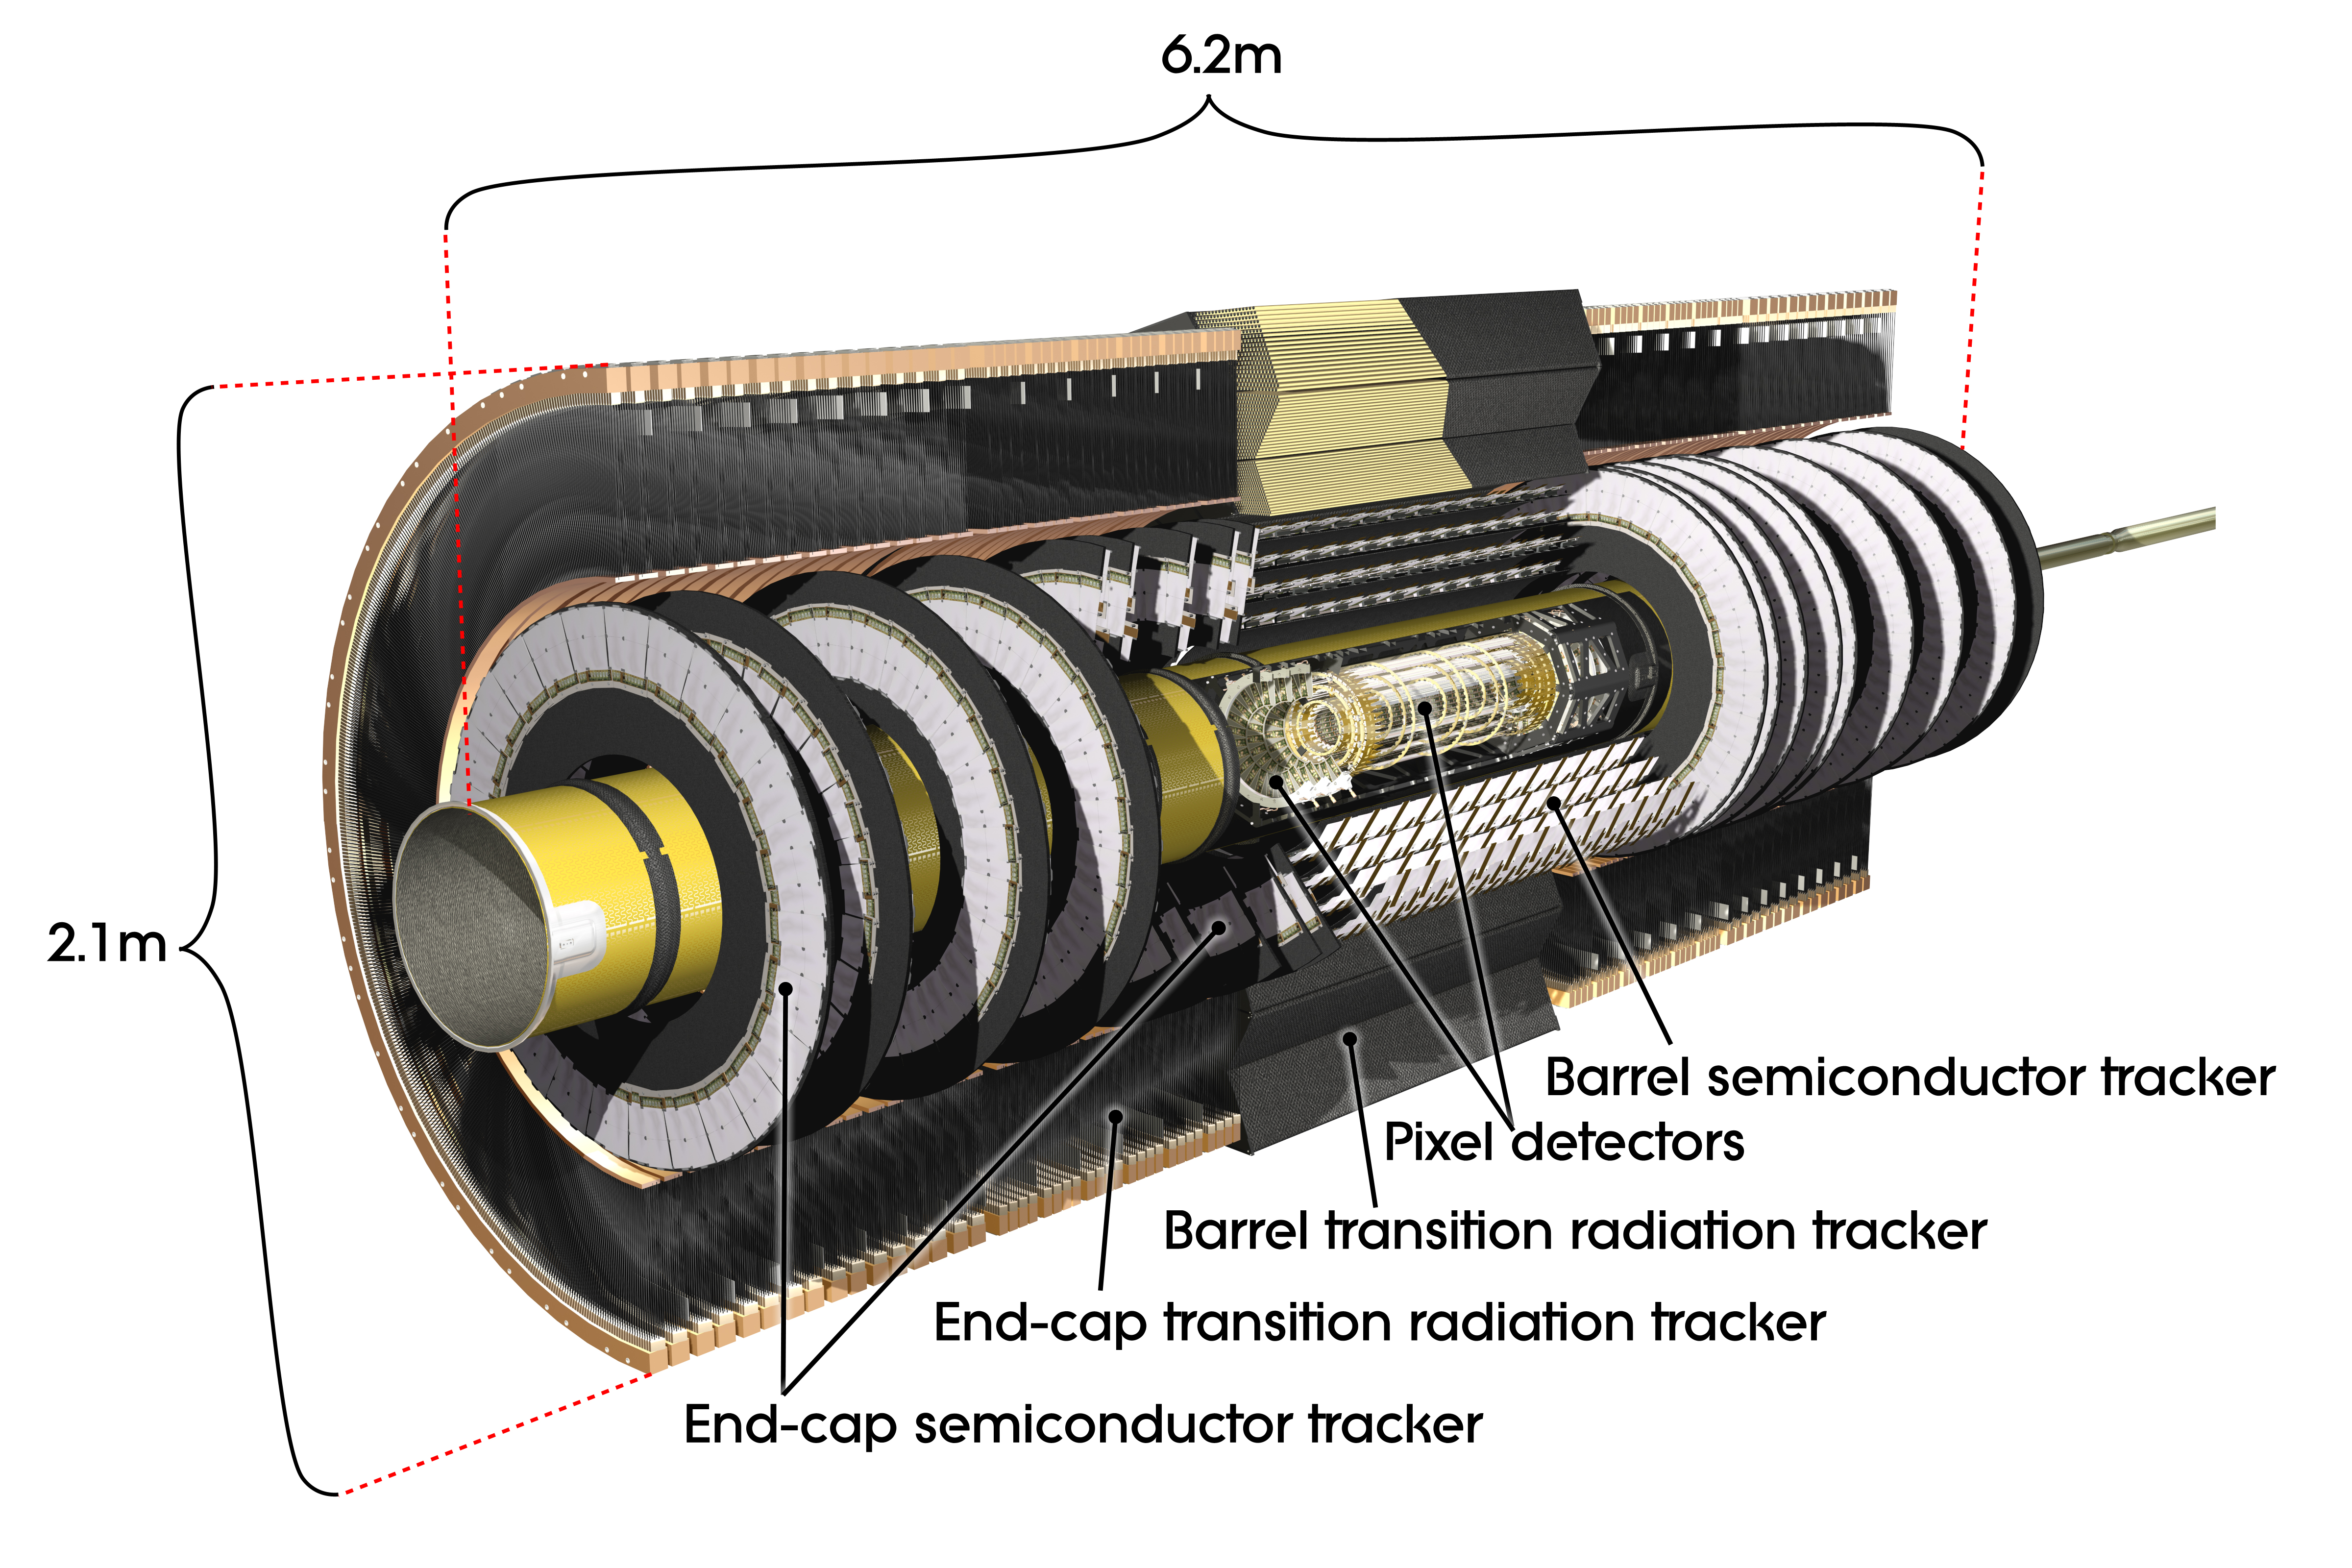
\includegraphics[clip, width=7cm]{fig/2/inner_detectoer1.jpg}
        \vspace{10pt}
        \subcaption{内部飛跡検出器の概略図}
        \label{fig:内部飛跡検出器の概略図1}
    \end{minipage}
    \hfill
    \begin{minipage}[b]{0.5\linewidth}
        \centering
        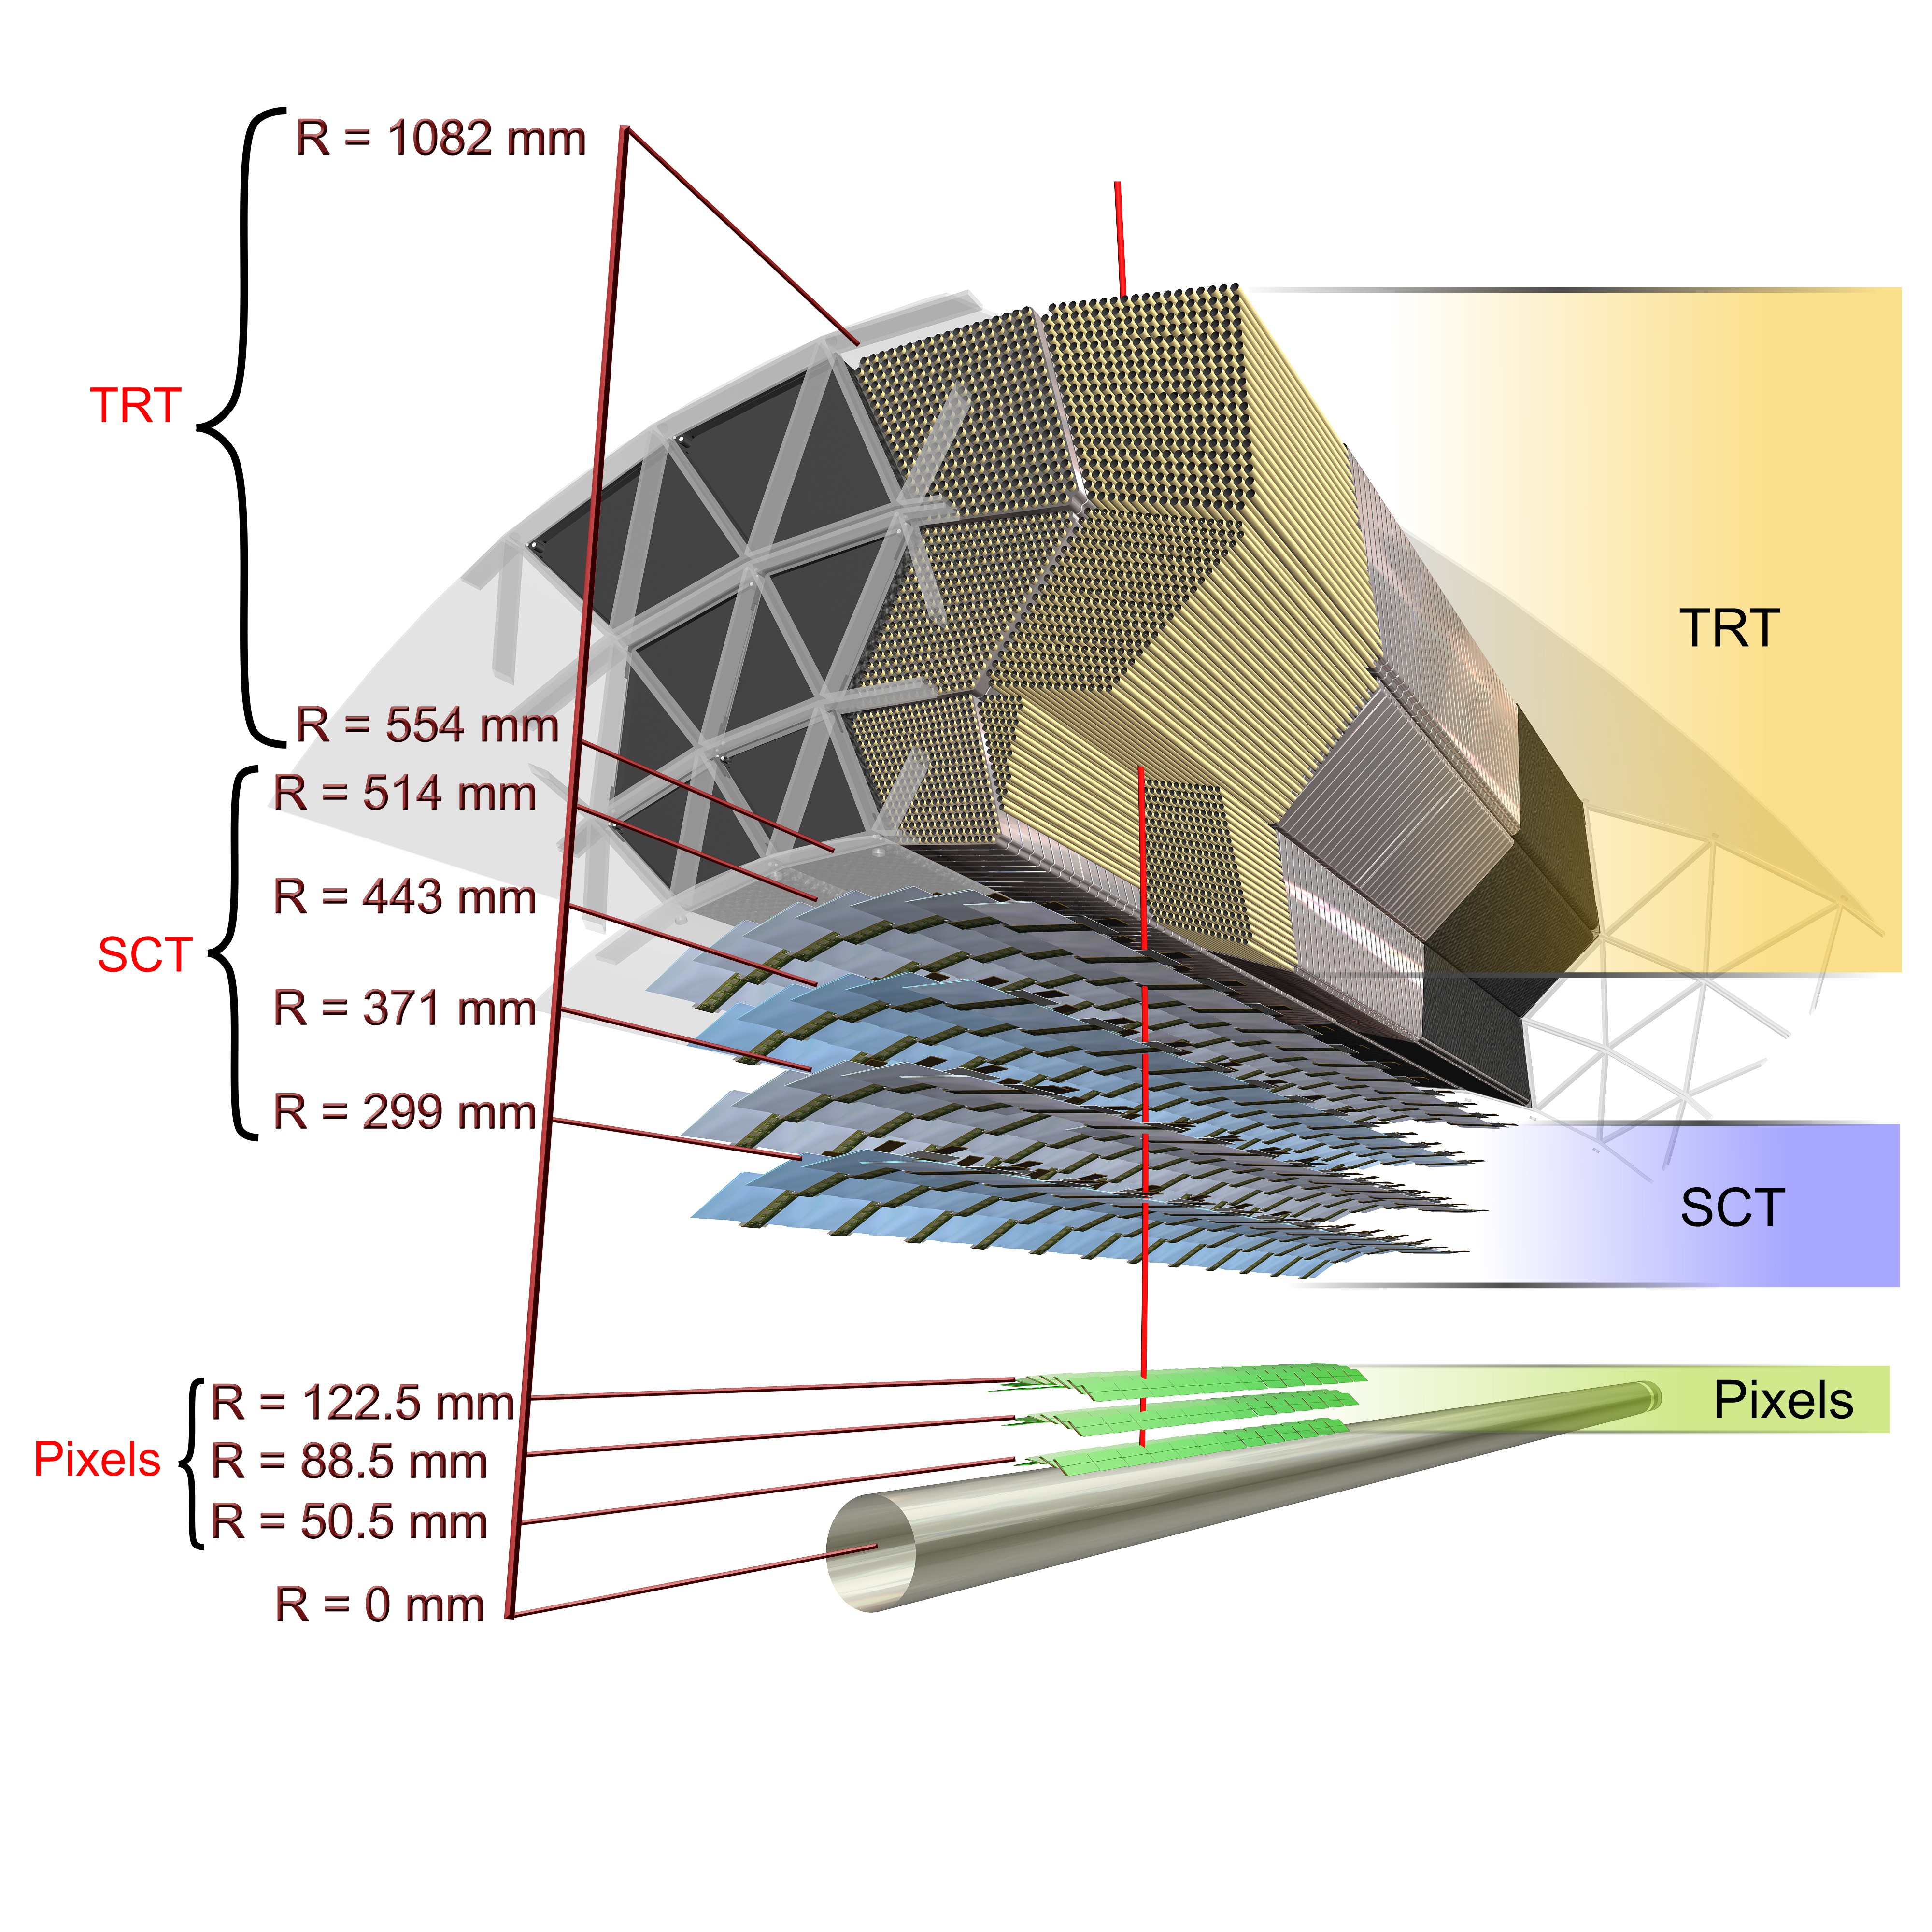
\includegraphics[clip, width=6cm]{fig/2/inner_detector2.jpg}
        \vspace{10pt}
        \subcaption{内部飛跡検出器の概略図}
        \label{fig:内部飛跡検出器の概略図2}
    \end{minipage}
    \caption{内部飛跡検出器}
    \label{fig:内部飛跡検出器}
\end{figure}



\subsection{カロリメータ}
カロリメータは、内部飛跡検出器の外側に設置されており、LHCでの陽子衝突で生成された粒子のエネルギー及び位置を測定する役割を担っている。
ATLAS検出器に設置されているカロリメータは、吸収層と検出層からなるサンプリングカロリメータであり、高密度物質の吸収層で粒子シャワーを起こし、検出層で電気信号に変えることで粒子の同定を行っている。
ATLASのカロリメータは、電磁カロリメータとハドロンカロリメータの2種類設置されている。

\subsubsection{・電磁カロリメータ}
電磁カロリーメーターは、$|\eta|<1.5$をカバーするバレルカロリメータと、$1.4<|\eta|<3.4$をカバーするエンドキャプカロリメータに分かれている。
バレル部とエンドキャプ部ともに、吸収層の鉛と検出層の液体アルゴンで構成されたカロリメータであり、電磁相互作用を起こす光子や電子のエネルギーと位置を測定する役割を担っている。

\subsubsection{・ハドロンカロリメータ}
ハドロンカロリメータは電磁カロリメータの外側に設置されており、タイルカロリーメータ、エンドキャップカロリーメータ、フォワードカロリーメータの3つに分類され、それぞれ異なる$|\eta=$範囲をカバーする。バレル部では、鉛と

\subsection{ミューオンスペクトロメータ}
\label{section2-2-4}

\subsubsection{・Resisitive Plate Chamber (RPC)}
\subsubsection{・New Small Wheel (NSW)}
\subsubsection{・Thin Gap Chambers (TGC)}
TGC は磁場領域より内側に EI (Endcap Inner) と呼ばれるステーション、磁場領域より外側に M1、M2、M3 (Middle 1,2,3) と呼ばれる 3 つのサブステーションが配置されている。磁場領域より外側にある M1 ステーションは TGC Triplet で構成されており、M2、M3 ステーションは TGC Doublet で構成されている。
M1、M2、M3 のヒット情報をトリガー判定に使用し、M3 はミューオントリガーの位置情報を決定するための基準として用いられているため、Pivot plane と呼ばれている。
磁場領域より内側にある EI ステーションは TGC Doublet で構成されており、これは EI チェンバーはトロイド磁石と干渉しないように配置されているため、図  のように一部の φ 領域のみをカバーしている。。TGC-EI のヒット情報を TGC-BW の飛跡情報とコインシデンスをとるために用いる。

\subsubsection{・Monitored Drift Tube (MDT)}
\subsubsection{・small-strip TGC (sTGC)}
\subsubsection{・Micromegas (MM)}









